\begin{document}

\maketitle
\begin{frame}{Outline}
\setcounter{tocdepth}{1}
\tableofcontents
\end{frame}

\section{Counter-Reformation}
\label{sec-1}
\begin{frame}[label=sec-1-1]{5 themes}
\begin{block}{Humanity and Divinity of Christ:}\pause
\begin{enumerate}
\item how fit the Catholic humanists in this?\pause
\end{enumerate}
\end{block}

\begin{block}{Reason and revelation: (What is true? Path to salvation?)}\pause
\begin{enumerate}
\item cf. bible and tradition vs. bible alone\pause
\end{enumerate}
\end{block}

\begin{block}{Works and Grace:}\pause
\begin{enumerate}
\item maintaining a tension,
\item cp. Contarini with similar exp. to Luther\pause
\end{enumerate}
\end{block}
\end{frame}

\begin{frame}[label=sec-1-2]{}
\begin{block}{Spirit and Structure: canons and ``reforms'' aimed at structure,}\pause
\begin{enumerate}
\item cf. also the turmoil over Carmelites\pause
\end{enumerate}
\end{block}

\begin{block}{Church and State:}\pause
\begin{enumerate}
\item nb that German Lutherans overthrew state authority, tradition that state followed ruler,
\item Rome pretensions to the Roman Empire (left over from high middle ages synthesis)
\end{enumerate}
\end{block}
\end{frame}
\section{Gods-governance}
\label{sec-2}
\begin{frame}[label=sec-2-1]{Geneva}
\begin{itemize}[<+->]
\item Europe being divided up
\item Radical reformation in pockets
\item Calvin inherited what Zwingli had begun
\item looked on as ``the Protestant Rome''
\end{itemize}
\end{frame}

\begin{frame}[label=sec-2-2]{Calvin}
\begin{columns}
\begin{column}{.5\textwidth}
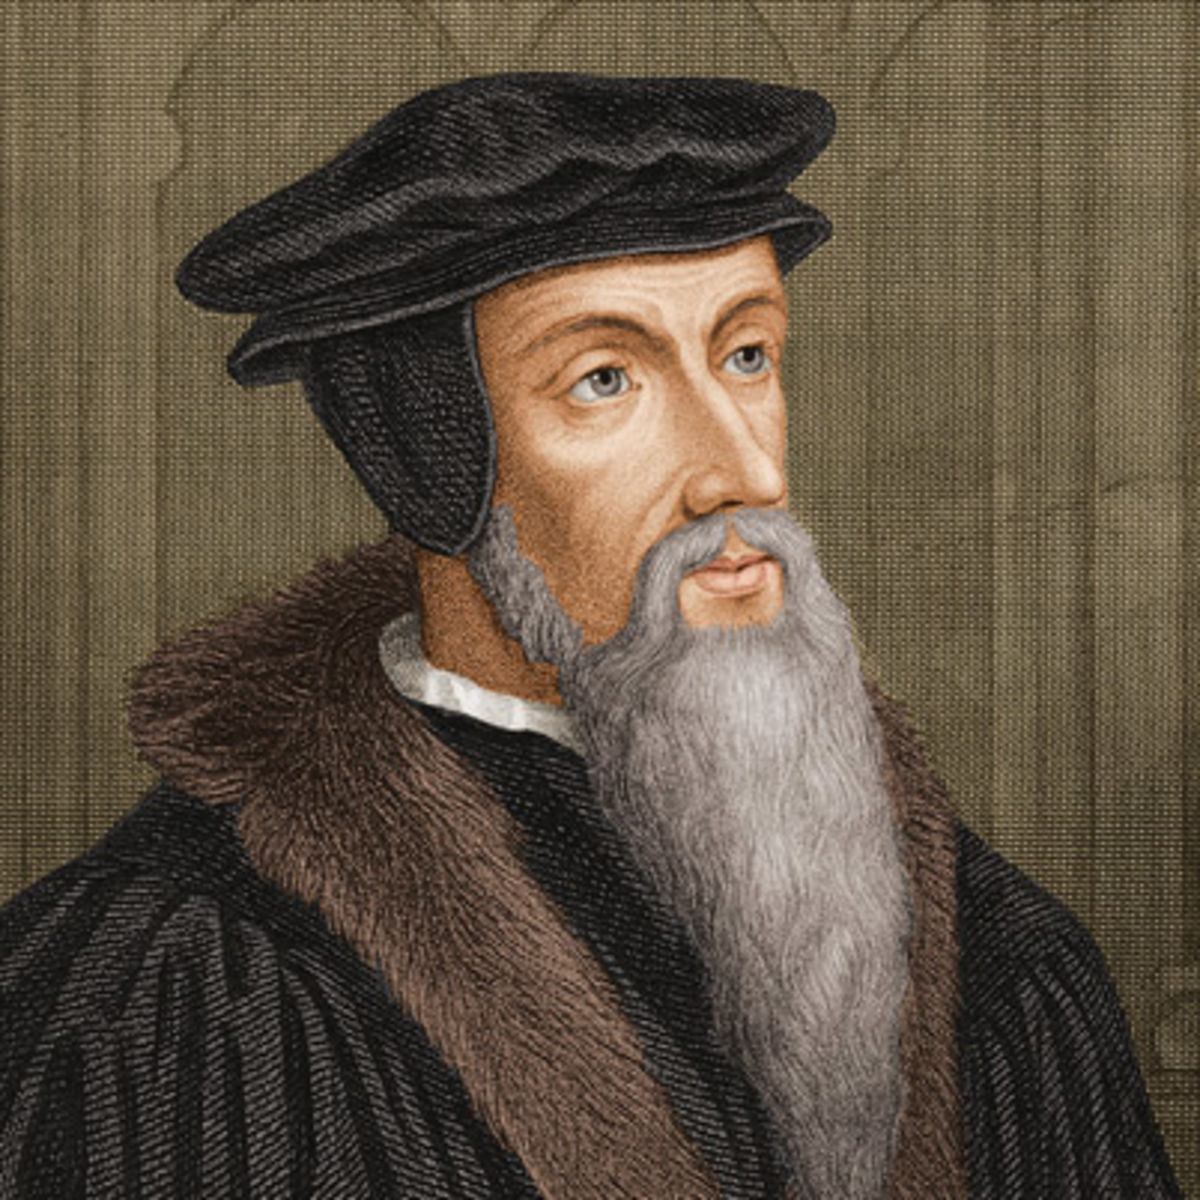
\includegraphics[width=.9\linewidth]{./img/john-calvin.jpg}
\end{column}

\begin{column}{.5\textwidth}
\url{https://prezi.com/ympfwolg3_no/john-calvin-the-greatest-exegete-of-the-reformation/}
\end{column}
\end{columns}
\end{frame}

\begin{frame}[label=sec-2-3]{Emphasis}
\begin{itemize}[<+->]
\item where Luther's emphasis on grace and justification
\item Calvin on covenant (in the lineage of Abraham)
\item the government of society bound up with notion of covenant
\item a ``civil'' use of law as well as ``theological'' (188)
\end{itemize}
\end{frame}

\begin{frame}[label=sec-2-4]{questions/focus}
\begin{itemize}[<+->]
\item ``reform'' as in ``reformed life''
\item organizing society, community
\item what is community?
\item 39 articles
\item ``Puritans''
\end{itemize}
\end{frame}

\begin{frame}[label=sec-2-5]{epithoughts}
\begin{itemize}[<+->]
\item ``Calvinist in polity'' -- huge influence on English world
\item Knox and Calvin and the ``reformed'' tradition
\item Calvin retreating from France to Geneva
\item reading Calvin elicits not an emotional response but a cumulative one from the systematic presentation p 188
\end{itemize}
\end{frame}

\begin{frame}[label=sec-2-6]{}
\begin{itemize}[<+->]
\item response to (free) grace is a \alert{reformed} life (thus the name)
\item in contrast to Luther's distinction between law and gospel, Calvin thought we stood in the same convenant as Abraham (189)
\item ``Reflections on how we come to be saved led to the doctrine of predestination (189 ff.)
\item \url{https://en.wikipedia.org/wiki/The_Private_Memoirs_and_Confessions_of_a_Justified_Sinner}
\item theology of sacraments: cf. \alert{Martin Bucer} (large influence)
\begin{itemize}
\item sought position between Luther and Zwingli
\end{itemize}
\end{itemize}
\end{frame}
\begin{frame}[label=sec-2-7]{Include for Wed. readings}
\begin{itemize}
\item Westminster confession
\item 39 articles
\end{itemize}
\begin{block}{Cp these two influences from Reformed tradition}
\end{block}
\end{frame}
% Emacs 24.3.1 (Org mode 8.2.3c)
\end{document}
